\documentclass[11pt]{amsart}
\usepackage{geometry}                % See geometry.pdf to learn the layout options. There are lots.
\geometry{letterpaper}                   % ... or a4paper or a5paper or ... 
%\geometry{landscape}                % Activate for for rotated page geometry
%\usepackage[parfill]{parskip}    % Activate to begin paragraphs with an empty line rather than an indent
\usepackage{graphicx}
\usepackage{amssymb}
\usepackage{epstopdf}
\DeclareGraphicsRule{.tif}{png}{.png}{`convert #1 `dirname #1`/`basename #1 .tif`.png}

\title{D. Paillard's Conceptual Climate Model (\emph{Nature} 1998)}
\author{ }
%\date{}                                           % Activate to display a given date or no date

\begin{document}
\maketitle
\section{About the Models}
These models were created to explain the glacial-interglacial cycles within the framework of the orbital perturbations affecting incoming solar radiation, together with the feedbacks related to the Earth's ice sheets.  

The first is a static model that changes states when thresholds are reached.  These thresholds are parameters in the model, and the states are \emph{i} (interglacial), \emph{g} (moderate glaciation), and \emph{G} (full glaciation).  The only transitions that are allowed are \emph{i}-\emph{g}, \emph{g-G} and \emph{G-i}, and all of these transitions take place when the insolation (read in at model run time) satisfies certain conditions related to each threshold.  See the figure below for a schematic diagram of the transitions that take place.

The second model is continuous in the extent of the ice sheet volume, and is otherwise just like the first static model. There are two time-related parameters in this model which can be tuned to match the data.

The insolation is provided by the file \texttt{ins\_65N\_July.txt}, which is the average insolation for the month of July at a latitude of 65 degrees north and is taken from Berger et al (1991).  The plots of the oxygen isotope stacks, which are a proxy for surface temperature, are taken from Bassinot et al (1994).

\section{Running the Model}
To run the models without changing parameters, simply type \texttt{paillard\_steady\_run} at the command line for the static model, or \texttt{paillard\_conts\_run} for the continuous time model.  The model will display three panels:  the insolation, normalized to mean 0 and unit variance, the ice volume, and the oxygen isotope stack.  To change parameters, edit the \texttt{paillard\_parameters.m} file, which has a description of each parameter in the comments at the beginning of the file.

Also included are the insolation file (\texttt{ins\_65N\_July.txt}) and the oxygen isotope stack file (\texttt{bassinot.txt}), but these should be considered as data and not altered.  The model is attempting to use the insolation data to simulate the oxygen isotope stack data.

\section{Reference}
\noindent Paillard, D. "The Timing of Pleistocene glaciations from a simple multiple-state climate model." \emph{Nature}.  Vol 391.  22-Jan-1998.  pp 378-381.\\
\\
\noindent Berger, A. and Loutre M.F.  "Insolation values for the climate of the last 10 million years."  \emph{Quaternary Sciences Review}, Vol 10, No. 4, pp. 297-317, 1991.\\
\\
\noindent Bassinot, FC et al. (1994): A low-latitude Upper Pleistocene oxygen isotope stack, doi:10.1594/PANGAEA.715006.\\
\indent Supplement to: Bassinot, Frank C; Labeyrie, Laurent; Vincent, Edith; Quidelleur, Xavier; Shackleton, Nicholas J; Lancelot, Yves (1994): The astronomical theory of climate and the age of the Brunhes-Matuyama magnetic reversal, Earth and Planetary Science Letters, 126(1-3), 91-108, doi:10.1016/0012-821X(94)90244-5
\\ \\ \\ \\ \\
\begin{figure}[h]
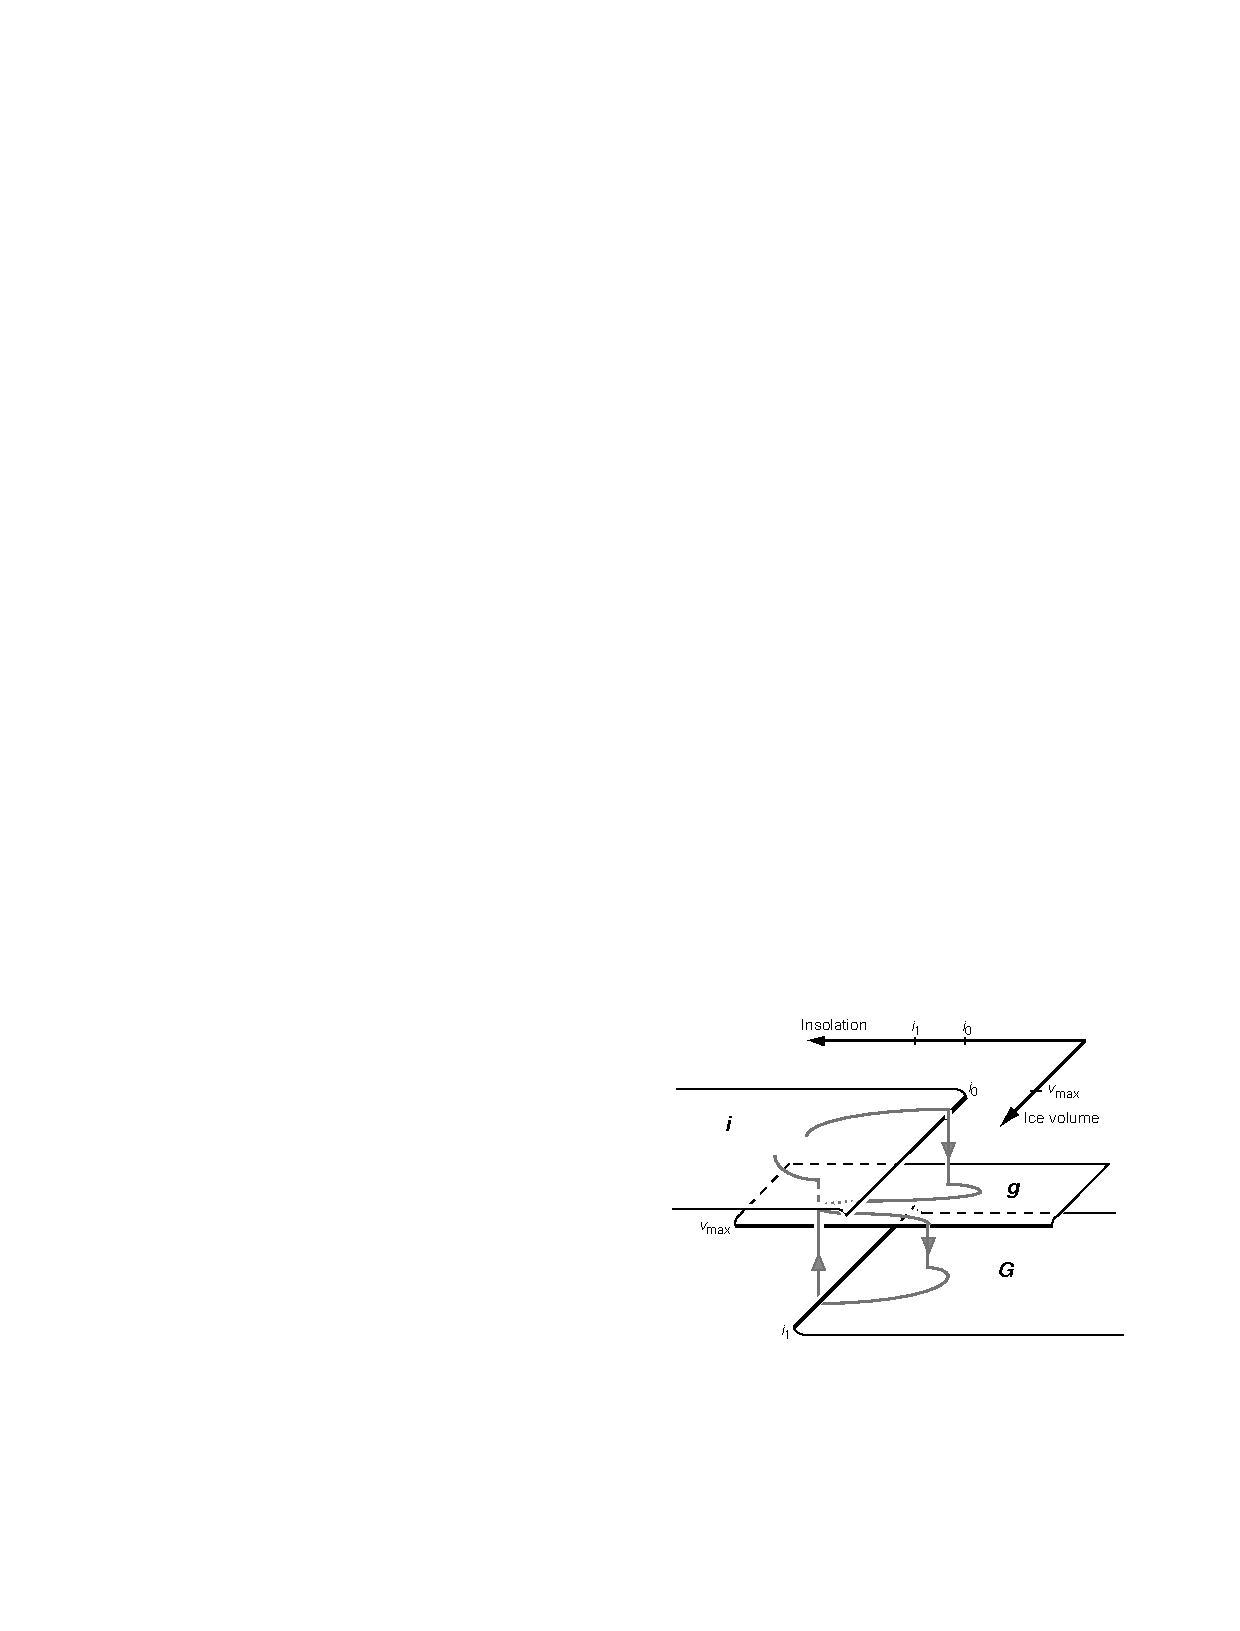
\includegraphics[scale=1.0]{paillard_model_cartoon.pdf}
\caption{Schematic of Model States, Transitions and Thresholds from Paillard (1998)}
\end{figure}
\end{document}  